\documentclass{report}
\usepackage[utf8]{inputenc}
\usepackage[english]{babel}
\usepackage{graphicx}
\usepackage{amsmath}
\usepackage{parskip}
\parskip=2\baselineskip \advance\parskip by 0pt plus 1pt

\newcommand{\analysis}{the \href{http://analysis.sns.gov}{Analysis} machine}

\newcommand{\cmd}[1]{\texttt{#1}}
\newcommand{\addiecmd}{\cmd{fastgr}}

\newcommand{\fileio}[1]{\texttt{#1}} 
\newcommand{\iptsPrint}{\fileio{/SNS/NOM/IPTS-<your experiment ID>}}

\newcommand{\guicmd}[1]{\textbf{\textit{#1}}}
 
\newcommand{\snspowderreduction}{\href{http://docs.mantidproject.org/nightly/algorithms/SNSPowderReduction-v1.html}{SNSPowderReduction}}
 
\usepackage[pdfpagelabels]{hyperref}
\hypersetup{
    colorlinks=true,
    linkcolor=blue,
    filecolor=magenta,      
    urlcolor=red,
}
 
\urlstyle{same}
 
\begin{document}

{\let\cleardoublep
\clearpage 
\begin{titlepage}
	\centering
	\includegraphics[width=0.6\textwidth]{graphics/joke_image.jpg}\par\vspace{1cm}
	\vspace{2cm}
	{\huge\bfseries ADDIE User Manual\par}
	{\LARGE\bfseries\itshape ADvanced DIffraction Environment\par}
	\vspace{1cm}
	{\Large\bfseries\ Data reduction software for NOMAD\par}
	\vfill
	{\large\bfseries \today{} version \par}
\end{titlepage}
 

 \tableofcontents
 \addtocontents{toc}{~\hfill\textbf{Page}\par}

}

\chapter{Introduction}
\section{What is ADDIE}
The ADvanced DIffraction Environment (ADDIE) is User software for 
reducing and analyzing data on the  
\href{http://https://neutrons.ornl.gov/nomad}{Nanoscale Ordered MAterials Diffractometer}  (NOMAD)  instrument at the \href{https://neutrons.ornl.gov/sns}{Spallation Neuron Source} (SNS). 
Now, with a full plate of acronyms, let's begin.


ADDIE provides a graphical user interface (GUI) to interact with the 
underlying data reduction software. ADDIE aims to guide the workflow to 
go from launching the reduction of raw neutron data to provided processed 
individual runs, post-processing of these individual runs  by applying 
optional corrections and summations, finally to visualization and 
output of the diffraction and pair distribution function data. 

ADDIE in pre-installed on the Analysis cluster at the SNS 
(\url{http://analysis.sns.gov}). Instructions are provided for Neutron Sciences users 
to setup the Remote Desktop capablities to view, analyze and download your data 
from anywhere you go. Options are provided Windows, Mac, and Linux. 
Also, contact support information is provided in the case of 
any issues or needed troubleshooting.

ADDIE is also avaible open-source. 
Please contact your Local Contact from NOMAD if you would like to 
know more about the repository (or to contribute!)
\section{Using ADDIE}

ADDIE development has been funded by the 
\href{https://www.energy.gov/}{US Department of Energy} (DOE). 

If you use ADDIE results in your published work, please cite the following papers:

(INSERT - ADDIE paper)
(INSERT - other reduction dependencies - Mantid, GUDRUN, etc.)

For any of the following features for your published work, please cite the associated papers:

(INSERT - specific feature papers)

From the following, you can download a \href{http://https://neutrons.ornl.gov/nomad}{BibTex file with all citations}.


 
\chapter{Getting Started}
\section{Background}

What does ADDIE actually do during data reduction? For each run, we must have the following measurements for data reduction:

\begin{equation} \label{eq_intensities}
\begin{split}
I_{sample}  & = \text{sample intensity} \\
I_{C}  & = \text{sample container intensity} \\
I_{Cb} & = \text{container background intensity} \\
I_{V}  & = \text{vanadium intensity} \\
I_{Vb} & = \text{vanadium background intensity} 
\end{split}
\end{equation}

Why all these measurements for a single run? We want to measure only the coherent sample scattering ($I_{sample}^{coh}$). Unfortunately, we cannot suspend the sample in space inside the instrument. We must have a sample container. Thus, we measure the empty sample container intensity ($I_{C}$) in the instrument to subtract this from the sample scattering intensity ($I_{sample}$). Yet, we can have many different types of "containers" (i.e. sample environments such as a furnace or cryostat, vanadium cans, quartz tubes, tubes in cans, etc.) Therefore, we must correct "from the outside in" where we subtract a completely empty instrument from the outermost containment scattering intensity, then subtract this from the next layer of containment and continue till we reach the sample subtracted ($I_{sample}$) from this collective background ($I_{C} + I_{Cb}$).  Also, we do not know the exact beam profile to put the sample scattering intensity on an absolute scale. For this, we use vanadium to normalize the sample scattering intensity to extract the coherent scattering ($I_{sample}^{coh}$) from the incoherent scattering ($I_{sample}^{inc}$) on an absolute scale. 

Why vanadium for normalization? We use vanadium for a few different reasons. 1) Vanadium has a small coherent scattering length but is a great incoherent scattering material. Thus, it does not contain large Bragg reflections in its profile that would have to be removed but provides a well-defined total beam profile. 2) Vanadium is a solid metal with well known density and stable without a container. 3) The large mass of vanadium atoms reduces the need to correct for inelastic scattering effects.

What else before we get our coherent sample intensity? Last, we must take into account the loss of intensity of the neutron beam as it passes through every material present in the experiment. To some degree, the sample, container, and vanadium will all attenuate the neutron beam. Ignoring the sample attenuation, we have: 

\begin{equation} \label{eq_reduction}
\begin{split}
I_{sample}^{coh} & = \frac{I_{sample}-\alpha_c (I_{C}-I_{Cb})}{\alpha_v(I_{V}-I_{Vb})}  
\end{split}
\end{equation}

From the coherent scattering, we have the total scattering structure function given as:

\begin{equation} \label{eq_reduction}
\begin{split}
S(Q) - 1 & = \frac {\frac{I_{sample}^{coh}}{N} - \langle b^2 \rangle }{{{\langle b \rangle}^2 }} \\
         & = \frac {\frac{d \sigma}{d \Omega}  - \langle b^2 \rangle }{{{\langle b \rangle}^2 }} \\
         & = 
\end{split}
\end{equation}

where ${\langle b \rangle}^2$ and $\langle b^2 \rangle$ are the squared average and average squared scattering power of the sample where:

\begin{equation} \label{eq_reduction}
\begin{split}
\langle b \rangle = \frac {\sum_{i}^{N} b_{i}}{N}
\end{split}
\end{equation}


where $b_i$ is the scattering power of atom $i$ and $N$ is the total number of atoms in the sample.

The pair distribution function (PDF) is obtained from the Fourier transform of $S(Q)-1$:

\begin{equation} \label{eq_reduction}
\begin{split}
G(r) = \frac{2}{\pi} \int_{\inf}^{0} Q [S(Q)-1] \text{sin}(Qr) dQ
\end{split}
\end{equation}

\section{Specifics of NOMAD data reduction}

To obtain $S(Q)$ we using the following:

\begin{equation} \label{eq_reduction}
\begin{split}
S(Q) - 1 = \frac{\frac{I_{sample}^{coh}}{N} - I_{poly}}{I_poly}
\end{split}
\end{equation}

where 
\begin{equation} \label{eq_reduction}
I_{poly} = \begin{cases} 
      		\frac{\rho \sigma \}{} & x\leq 0 \\
      		\frac{100-x}{100} & 0\leq x\leq 100 \\
      		0 & 100\leq x 
		 \end{cases}
\end{equation}
\chapter{Quick Start Guide}

\textbf{Add abbreviated startup guide to this section. Distill what is in the rest of the manual}
\chapter{Workflow for Data Reduction}
Just a test
\section{Launch automatic data reduction of individual runs}


\subsection{Raw neutron event files}
Once the samples are in the beam, the experiment is setup, and you begin collecting data in runs, raw neutron events will begin being saved in files. Raw neutron events are every instance of a neutron being detected by a detector. 

For NOMAD at the SNS on \analysis, the saved files are NeXus files located in your IPTS folder under \iptsPrint/\fileio{nexus}. These are permanent files that cannot be edited or deleted. In these files are the neutron event data and also the metadata associated with the run (i.e. what temperature a probe is reading, what are the chopper settings, sample information). 

These raw neutron event files are what we reduce to get to the useful data for our material. This process is referred to as data reduction.

\subsubsection{Examining NeXus files}

You can examine the NeXus files from the command line of a terminal using \fileio{nxbrowse <NeXus filename>}. These files have a directory structure. You can \cmd{ls} to list the current level of the directory and use \cmd{cd} to enter a directory. All these files have the \fileio{entry} as the initial entry point. Then, if you \cmd{ls}, you will see that there are entries with the attributes \fileio{NX Group} and \fileio{NX Data}. For any entry with the attribute \fileio{NX Data}, you can use \cmd{read <entry>} to read the value of this entry. For any with the attribute \fileio{NX Group}, this is a sub-level directory associated with this entry. You can \cmd{cd} into the \fileio{NX Group} and then proceed with using \cmd{read}. To exit the NeXus file, you can use \cmd{exit} at any time to return to the terminal.



\subsection{Experiment Information Input}

ADDIE can be used to launch an automated data reduction, or autoreduction, of your sample runs as they complete and produce NeXus files. The autoreduction processes the NeXus files as they appear under your IPTS folder.

\subsubsection{Loading In the Experiment Information}

To setup the autoreduction, first launch ADDIE as described before. You will begin with the following screen with the autoreduction tab open:

\noindent\makebox[\textwidth]{\includegraphics[width=0.9\paperwidth]{graphics/tab1/tab1.png}}

Here, we input the run numbers for the necessary measurements specified in Equation \ref{eq_intensities} in order to create our reduced data, Equation \ref{eq_reduction}. To read in this data from an experiment input file (the \fileio{exp.ini} file), click on the \guicmd{Select Working Folder...} button at the top. You will be presented with a dialog box that will prompt you to select a working directory. It will begin with your current working directory, which you can see displayed at the top in the \guicmd{Look in:} field. If you are in your \iptsPrint directory, you should get something as below:

\noindent\makebox[\textwidth]{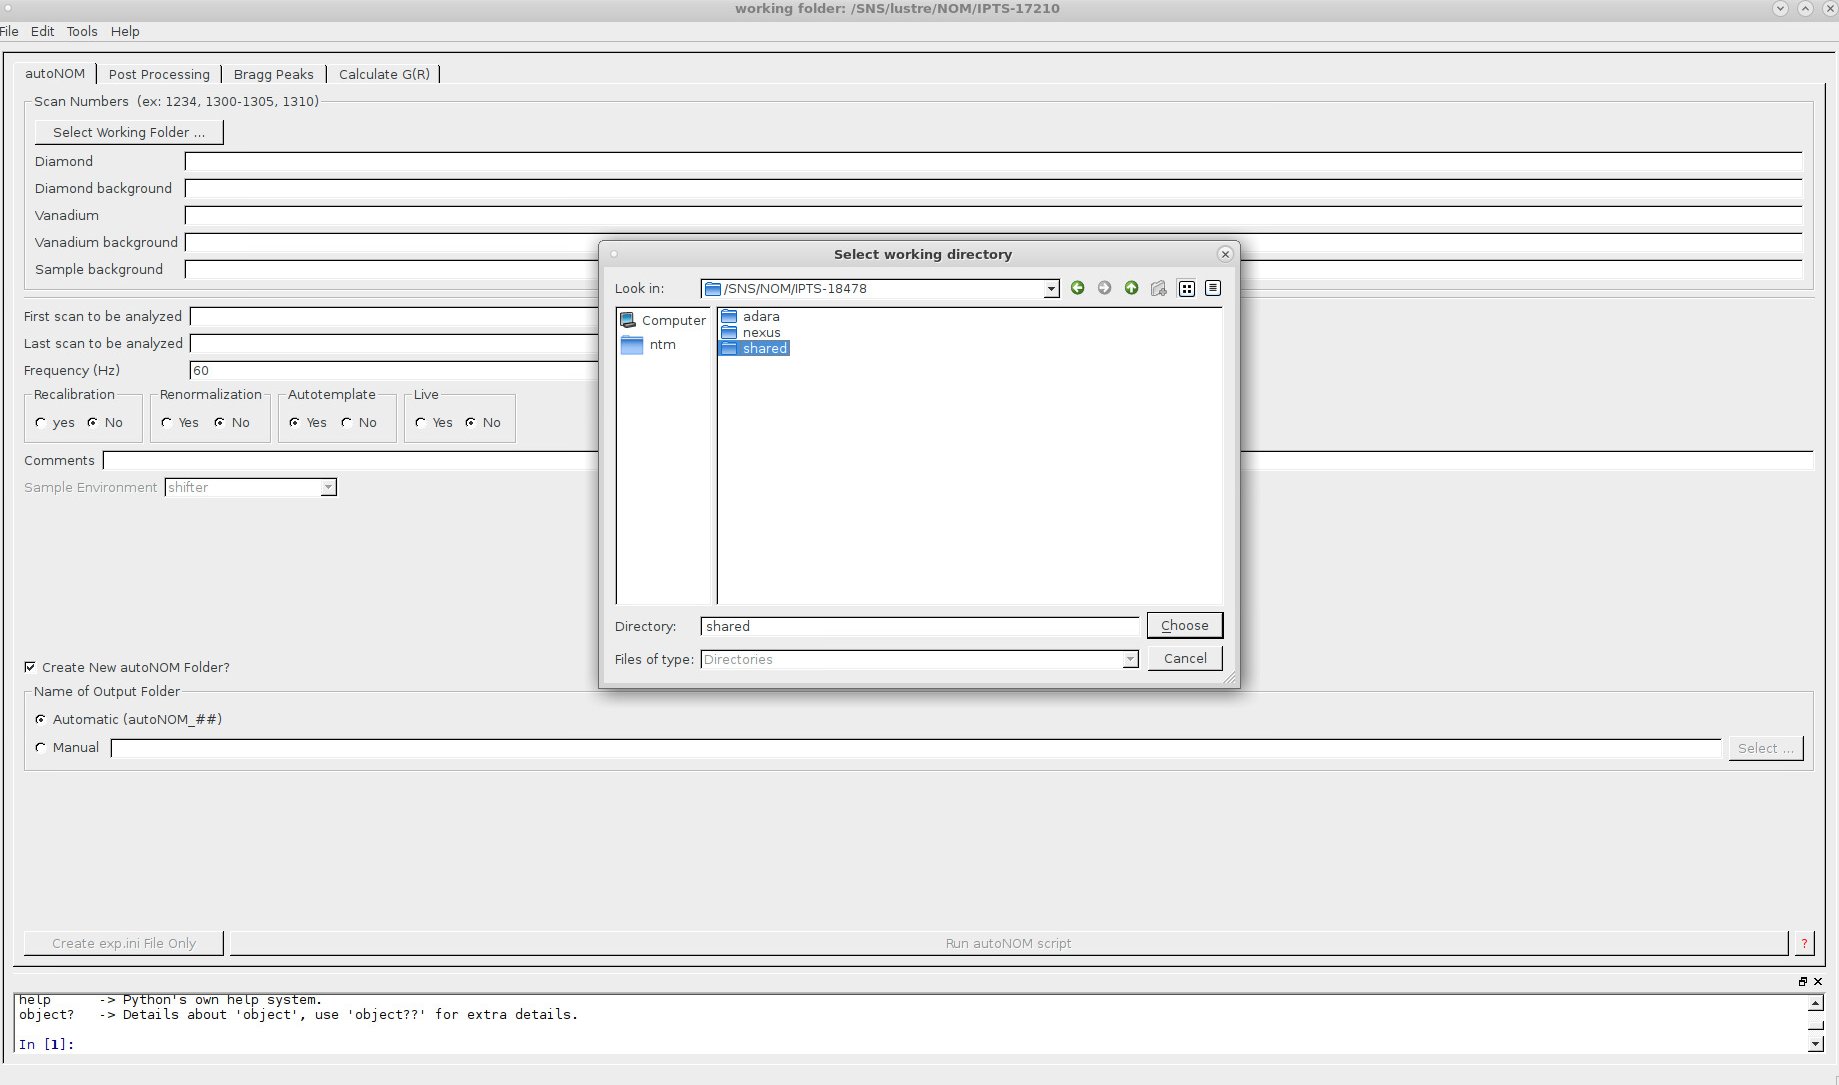
\includegraphics[width=0.9\paperwidth]{graphics/tab1/tab1_selectWorkingFolder_sharedFolder.png}}

This is the file directory structure of your IPTS. You can see the \fileio{nexus} directory where the raw neutron event files are stored, the \fileio{adara} directory (ADARA = Accelerating Data Acquisition, Reduction, and Analysis) for automated live reduction files, and the \fileio{shared} directory, which is a User workspace for the experiment. Double-click the \fileio{shared} directory and you will see something similar to the following:

\noindent\makebox[\textwidth]{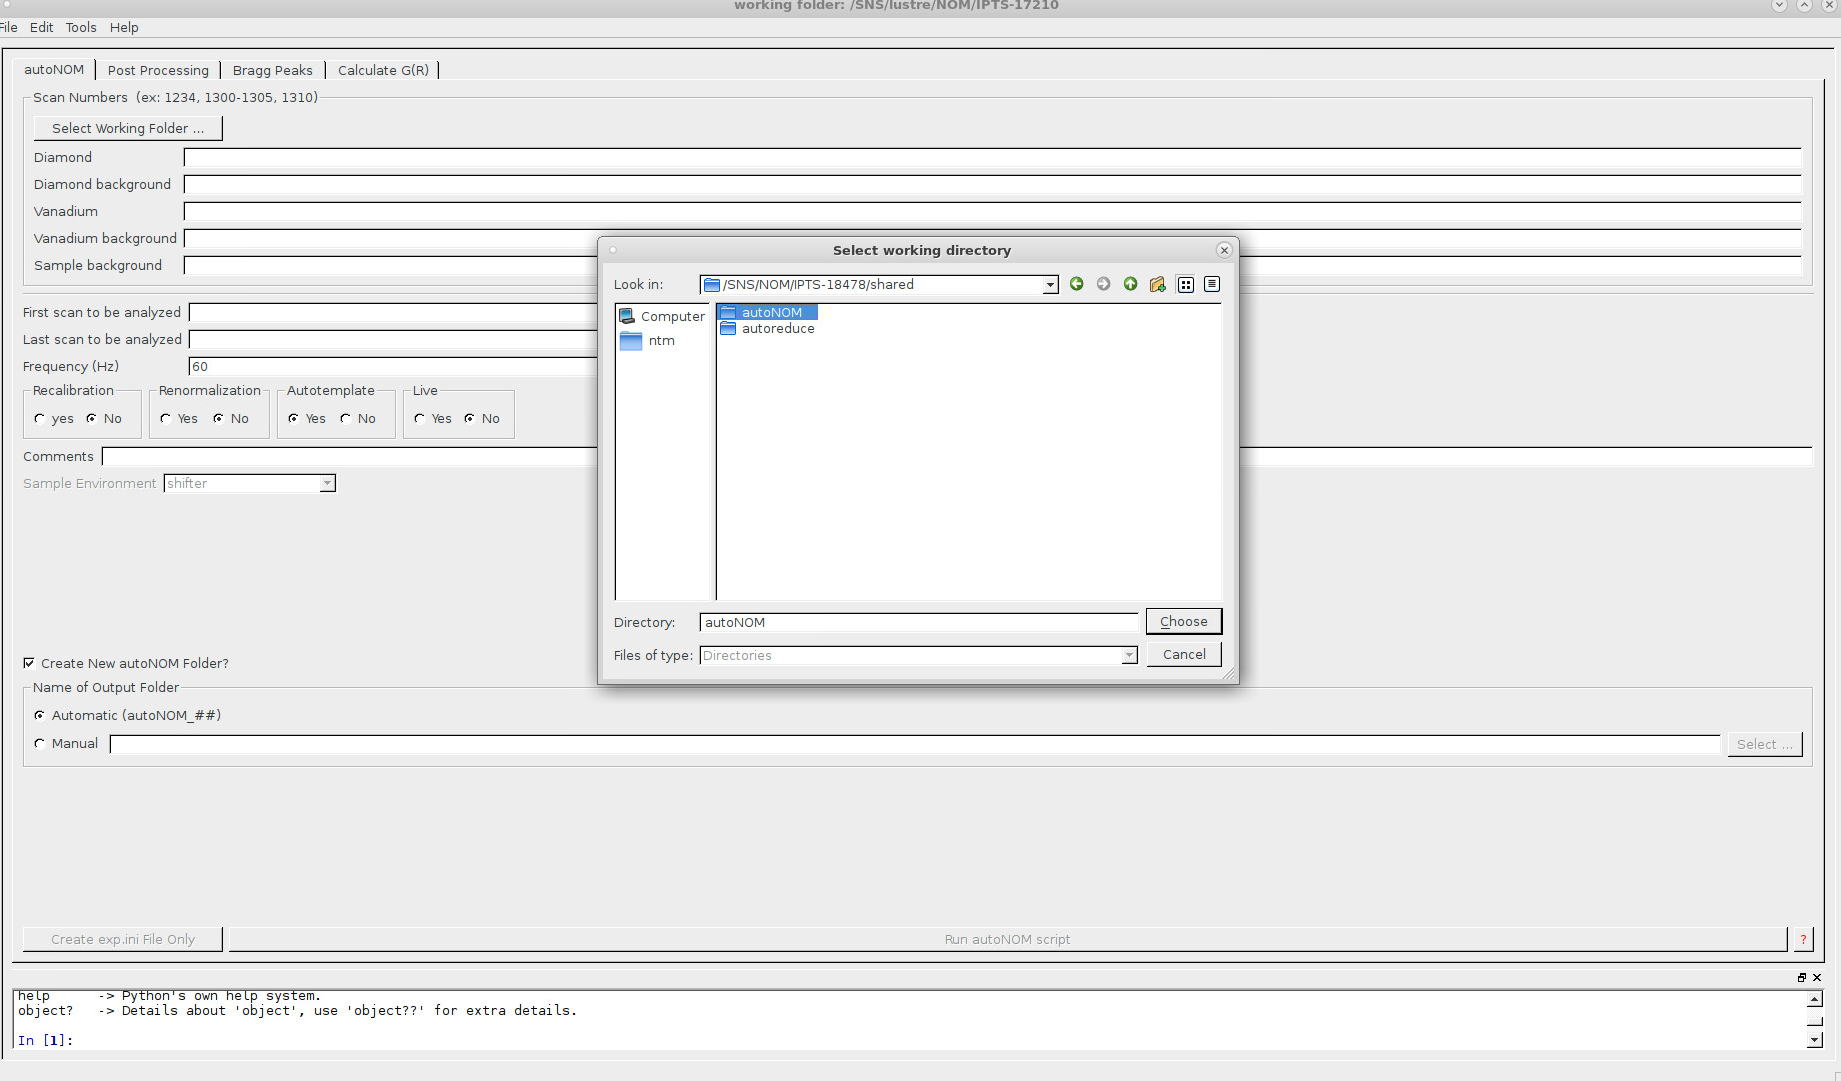
\includegraphics[width=0.9\paperwidth]{graphics/tab1/tab1_selectWorkingFolder_autoNOMfolder.png}}

Here, the \fileio{autoNOM} directory is where we will kick off the autoreduction of ADDIE. This will produce the \fileio{autoreduce} directory that you see above. This IPTS has already had the data reduction performed. If your IPTS has not yet had the data reduced, you may not see either of these directories. If the \fileio{autoNOM} directory does not exists, go to the terminal, get to the shared directory above ( \cmd{cd \iptsPrint/shared} ) and create it using the command: \cmd{mkdir autoNOM}. Once this directory exists, double-click the \fileio{autoNOM} directory. You will see something similar to the following:

 \noindent\makebox[\textwidth]{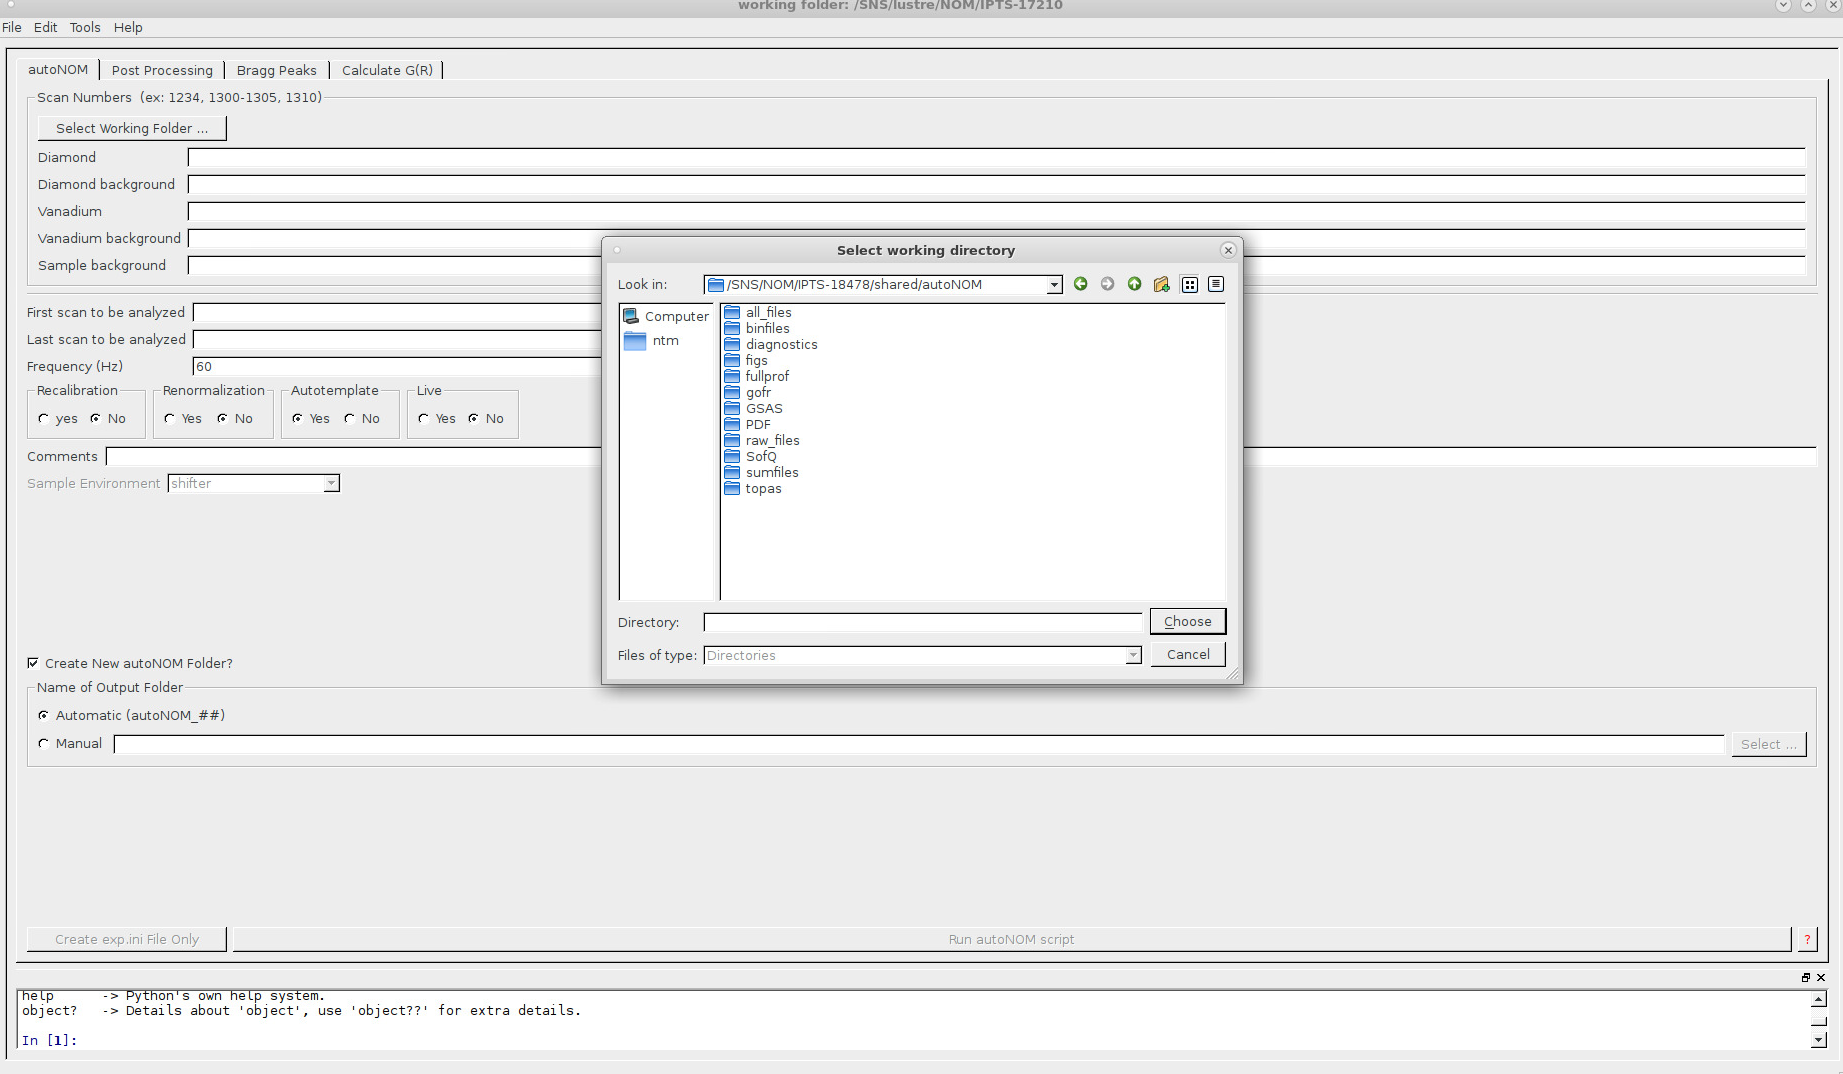
\includegraphics[width=0.9\paperwidth]{graphics/tab1/tab1_selectWorkingFolder.png}}
 
 Again, we have already launched data reduction in this IPTS so you see the directories that will be produced. For now, simply select \guicmd{Choose} on the bottom left. This will look for the experiment input file (the \fileio{exp.ini} file) in the current directory. If the file is found, the tab should populate with the experiment information in the file and look similar to the following:
 
  \noindent\makebox[\textwidth]{\includegraphics[width=0.9\paperwidth]{graphics/tab1/tab1_populated.png}}
  
If no experiment file was found, you will see the following next to the \guicmd{Select Working Folder...} button:

  \noindent\makebox[\textwidth]{\includegraphics[width=0.5\paperwidth]{graphics/tab1/tab1_selectWorkingFolder_error.png}}
  
If this occurs, you can fill in the necessary fields. Once you have these filled in, you can output an experiment input file using the \guicmd{Create exp.ini File Only} button. Yet, this file will be automatically created once we kick off the autoreduction. 

The experiment input file (\fileio{exp.ini} file) has the following format:

  \noindent\makebox[\textwidth]{\includegraphics[width=0.25\paperwidth]{graphics/tab1/tab1_experimentInputFile.png}}

\subsubsection{If No Experiment Information File Exists}

If you do not know these run numbers required to begin processing your data but you have measured them in your current IPTS, you can create a List of Scans file (a \fileio{los.txt} file) that has this information using the following command on the command line of a terminal:

\cmd{python /SNS/NOM/shared/autoNOM/stable/readtitles.py}

You can open this file (\fileio{los.txt} from ADDIE by going to the \guicmd{File} drop-down from the \guicmd{Menu} bar and selecting the \guicmd{Preview Ascii...} and selecting the \fileio{los.txt} file. You can optionally use a text editor (\fileio{gedit, vim, emacs}) from a terminal.

  \noindent\makebox[\textwidth]{\includegraphics[width=0.3\paperwidth]{graphics/dropdown/dropdown_file_previewAscii.png}}
  
  If you have any trouble with this step, please contact your Local Instrument Scientist Contact to help you get the necessary files. These can even be located in a directory you do not have access to, in which case, the Instrument Scientist can help assist you and ensure you have all the necessary files to launch the data reduction.
  

  
\subsection{Setting up Data Reduction}

At this point, you should have experiment information input into the tab similar to the following:

  \noindent\makebox[\textwidth]{\includegraphics[width=0.9\paperwidth]{graphics/tab1/tab1_populated.png}}
  
  
If you have questions about the run numbers (Diamond, Vanadium, Backgrounds, etc.) and what they are used for, please refer to Section \ref{sec_background} for an explanation. 

Settings:
\begin{itemize}

\item \guicmd{First scan to be analyzed}: we input the first run number of your IPTS. This can be found from the DAS where you setup the experiment and are controlling the instrument. It will be under \fileio{Run Information} as \fileio{Run Number}, similar to the following where the run number is 91566:

  \noindent\makebox[\textwidth]{\includegraphics[width=0.25\paperwidth]{graphics/das_runInformation.png}}
  
\item \guicmd{Last scan to be analyzed}: The last run to be analyzed. If you are running a "live" experiment, you can set this to an arbitrarily large run number. Only run numbers with associated NeXus files under the current IPTS will be found and reduced. 

\item \guicmd{Frequency}: Change the frequency mode of the data reduction. You can select from either 60 Hz (use every proton pulse that hits the target) or 30 Hz (use every other proton pulse). You can use the 30 Hz mode to use longer times-of-flight and thus longer wavelenths. Typically, we operate in the 60 Hz mode. 

\item \guicmd{Recalibration}: Either use the current calibration files present or re-perform calibration using the input Diamond run. If the re-calibration is set to \fileio{No} but no calibration files are found, it will automatically perform the calibration again. 

\item \guicmd{Renormalization}:   Either use the current normalization files present or re-perform calibration using the input Vanadium run. If the re-normalization is set to \fileio{No} but no normalization files are found, it will automatically perform the normalization again. 

\item \guicmd{Autotemplate}: Setup an organized directory structure under the autoNOM parent diretory. Always recommended and preferred.

\item \guicmd{Live}: Launch data reduction in either live mode where NeXus files will continuously be produced or in a post-processing mode where data reduction will stop once the last scan is analyzed. 

\item \guicmd{Commend}: This is a place to store a metadata comment about the experiment input information. Examples would be in what IPTS were the diamond and vanadium runs used from if they did not come from this ITPS, what was the sample environment, and any other information. This will be stored in the experiment input file (the \fileio{exp.ini} file).

\item \guicmd{Sample Environment} Specifies the sample environment. Used to determine if a calibration already exists for this sampel environment.

\item \guicmd{Creaete New autoNOM Folder?}: When data reduction is launched, this will create a new autoNOM directory and work within that folder. If you have already made an autoNOM directory, uncheck this box or you will have an autoNOM directory inside another autoNOM directory. You can let the autoNOM directory be automatically named sequentially or you can manually input the name of the directory.

\end{itemize}

\subsection{Launch Data Reduction}
Once the data reduction is setup and ready, you can kick off the automatic data reduction by pressing the \guicmd{Run autoNOM script} button. If everything is okay, you should see the Job Monitor window appear with the status of the job: 

  \noindent\makebox[\textwidth]{\includegraphics[width=0.9\paperwidth]{graphics/tab1/tab1_runAutoNOM_jobMonitor.png}}
  
If not running in "Live" mode, you will see a display of \guicmd{Done!} when the job is complete.

The Logbooks in the Job Monitor window display the output from log files that are saved and located in the \fileio{logs} directory under the parent autoNOM directory. Only the most recent Logbooks are displayed. The Logbook view is updated every 5 seconds by default. If you would like to pause the Logbook to scroll up and see the output, you can check the \guicmd{Pause Refresh Logbook} radio button at the bottom. Once you are done and want to refresh the Logbook, simply press the same button again to uncheck it.

If, at any time, you need to stop the data reduction, you can press the \guicmd{Abort!} button to kill all the running processes associated with the job. You will see a display of \guicmd{Killed!} when the job is finished aborting.

If the \guicmd{Run autoNOM script} button is greyed out and you cannot select it, something is missing from the data reduction setup. Press the question mark button located beside the \guicmd{Run autoNOM script} button and you will be shown what is missing in the pop-up Button Status window. Below, we have forgot the Diamond background:

  \noindent\makebox[\textwidth]{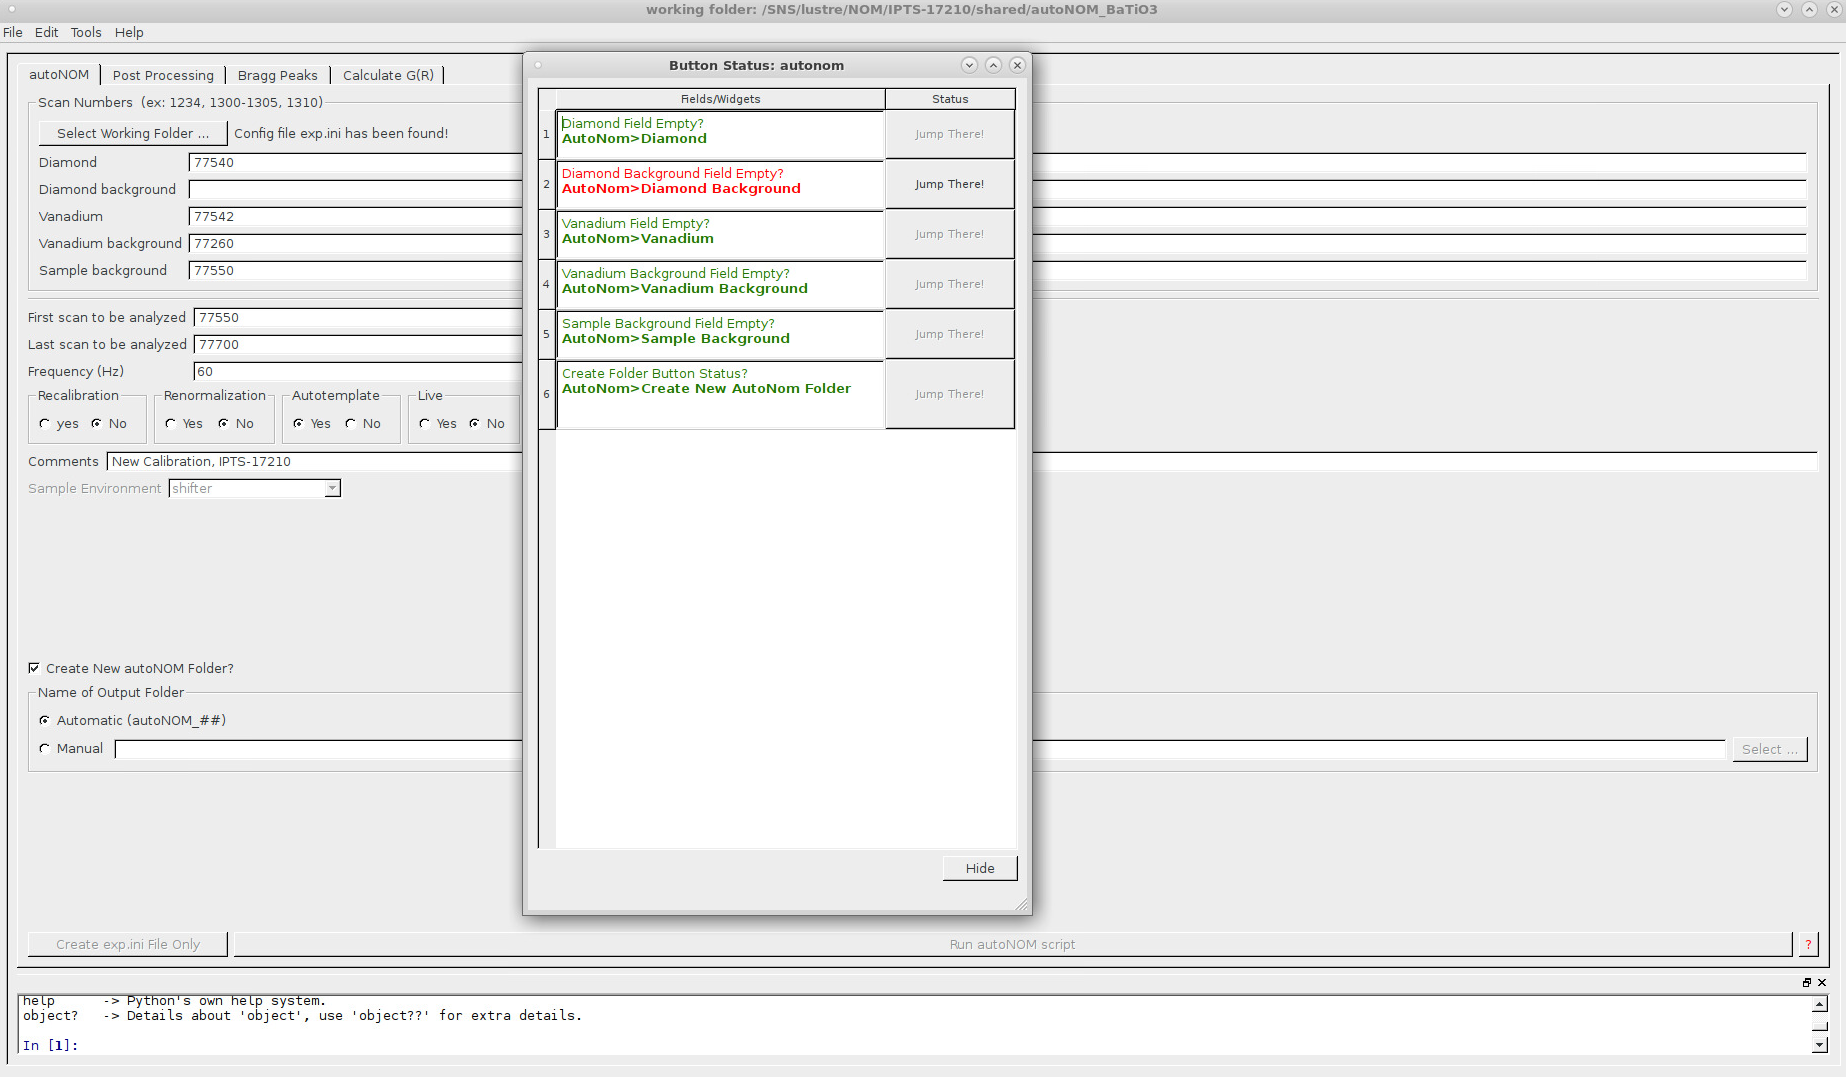
\includegraphics[width=0.9\paperwidth]{graphics/tab1/tab1_runAutoNOM_questionMark.png}}
  
\subsection{The directory structure}

When the data reduction is begun (and if the autotemplate options was chosen), the \fileio{autoNOM} directory will have the following directories with the described datasets:



 
 \begin{tabular} {|| p{3cm} | p{12cm} |} 
 \hline
 Directory & Contents  \\ [0.5ex] 
 \hline\hline
 all\_files & The generated IDL readable data files for individual scan number.  Users will not typically interact with “all” files. \\ 
 \hline
 binfiles & The IDL processing finle for generating Bragg and PDF data from “all” files.  Users will not typically interact with binfiles.
 \\
 \hline
 diagnostics & Diagnostics for the calibration performed.   Plots of various data quality metrics are provided.
\\
 \hline
 figs & A "scratch" place for the User to place various saved figures. \\
 \hline
 gofr & Contains small g(r), utilized by liquids and glass community. \\
 \hline
 GSAS & Contains diffraction patterns in GSAS (*.gsa)) and PDFgetN (*.getN) readable formats for the 6 default detector arrays of NOMAD. \\
 \hline
  fullprof & Contains diffraction patterns in Fullprof (*.dat) readable format for the 6 default detector arrays of NOMAD. \\
 logs & Logbook files for each process launched. Mainly used for debugging. Users will not typically interact with Logbooks.  \\
 \hline
 PDF & Contains G(r) or PDF of your samples,  in PDFgui format (*.gr)  \\
 \hline
 rietveld & Contains diffraction patterns in TOPAS (*.xye) and Fullprof (*.dat) readable formats for the 6 default detector arrays of NOMAD. Produced by Mantid instead of autoNOM if launched from \guicmd{Rietveld} sub-tab in \guicmd{Post-Processing} tab. \\
 \hline
 SofQ & ASCII file of S(Q)-1 \\
 \hline
 sumfiles & A "scratch" directory for the User to place summed files \\
 \hline
 topas & Contains diffraction patterns in TOPAS (*.xye) readable format for the 6 default detector arrays of NOMAD. \\ [1ex]
 \hline
\end{tabular} \label{table_directory_struct}




\subsection{Getting files from another IPTS}

If the diamond, vanadium, and background runs where processed in another, you can use the IPTS File Transfer tool to move over those files and bypass the need to repeat the calibration and normalization steps. \textbf{NOTE:} On \analysis, you must have the necessary permissions to access another IPTS. This may need to be performed by an Instrument Scientist with the correct permissions. If the runs exists in another IPTS but have not been processed yet, then you can proceed as normal. If you have the necessary permissions, calibration and normalization will continue as if those files where in your IPTS.

To transfer files from another IPTS, go to the \guicmd{Tools} drop-down of the \guicmd{Menu} bar and select \guicmd{IPTS Fil Transfer...}. You will be presented with the following dialog box:

  \noindent\makebox[\textwidth]{\includegraphics[width=0.9\paperwidth]{graphics/tab1/tab1_iptsFileTransfer.png}}
  
First, press the \guicmd{IPTS...} button to select the IPTS from the pop-up box. Here we are selecting IPTS-18314. Press \guicmd{Choose} once selected::

  \noindent\makebox[\textwidth]{\includegraphics[width=0.9\paperwidth]{graphics/tab1/tab1_iptsFileTransfer_selectIPTS.png}}
  
  
Then, press the \guicmd{autoNOM...} button in the \textbf{Source} section to select the specific autoNOM directory. From below, you can see that an IPTS can have multiple autoNOM directories. We are selecting the autoNOM\_2017A\_cryostat below. Press \guicmd{Choose} once selected:

  \noindent\makebox[\textwidth]{\includegraphics[width=0.9\paperwidth]{graphics/tab1/tab1_iptsFileTransfer_selectAutonomFrom.png}}
  
Finally, press the \guicmd{autoNOM...} button in the \textbf{Target} section to select where you will transfer the files. We are selecting the autoNOM\_new\_test directory below in IPTS-17210. Press \guicmd{Choose} once selected:

  \noindent\makebox[\textwidth]{\includegraphics[width=0.9\paperwidth]{graphics/tab1/tab1_iptsFileTransfer_selectAutonomTo.png}}
  
Now, you are ready to transfer. Press the \guicmd{Transfer Files} button and the transfer will start. the Job Monitor window should appear and let you know when the transfer is complete. This is usually a very quick transfer. 

  \noindent\makebox[\textwidth]{\includegraphics[width=0.9\paperwidth]{graphics/tab1/tab1_iptsFileTransfer_jobMonitor.png}}
\section{Post-Processing of runs}
\subsection{Load Runs into Table}
\subsection{Selection of Runs}
\subsection{Selection of Post-Processing}
\subsection{Launch Post-Processing}

\section{Visualize Bragg Diffraction}
\subsection{Load Bragg data}
\subsection{Adjust Graphs}

\section{Visualize S(Q) and G(r)}

As individual runs or post-processed runs are completed, the output files will be placed in their respective directories specified in Table \ref{table_directory_struct}. The S(Q) data is found in the \fileio{SofQ} directory and the real-space data is found in the \fileio{gofr} and \fileio{PDF}. 

To visualize and plot both sets of of data (reciprocal-space and real-space), we use the \guicmd{Calculate G(r)} tab shown below: 

\noindent\makebox[\textwidth]{\includegraphics[width=0.9\paperwidth]{graphics/tab4/tab4.png}}

A note on how the two plots work: When S(Q) data is loaded in, the Fourier transform is calculated automatically and the corresponding G(r) is displayed in the corresponding plot. Thus, ADDIE allows one to simultaneously view both the S(Q) and corresponding G(r) and also adjust and refine both datasets in an "on-the-fly" manner.

\subsection{Load S(Q) data}

First load in S(Q) datasests. Go to the top right and press the \guicmd{Load SQ} button. You should be presented with a file dialog similar to the one below:

\noindent\makebox[\textwidth]{\includegraphics[width=0.9\paperwidth]{graphics/tab4/tab4_loadSQ.png}}

If you are not in the \fileio{SofQ} directory, double-click the \fileio{SofQ} diretory to see the files that are available.  From here, you can select individual runs, labeled as \fileio{NOM\_<run number>SQ.dat} or you can select post-processed runs such as summed files, labeled as \fileio{NOM\_9999\_<given title>\_SQ.dat}.

You can also select multiple individual runs while holding the \cmd{Ctrl} key or you can select a span of runs by holding the \cmd{Shift} key while selecting the runs. Once the runs are selected, press the \guicmd{Open} button. For our example above, we get the following displayed:

\noindent\makebox[\textwidth]{\includegraphics[width=0.9\paperwidth]{graphics/tab4/tab4_loadSQ_afterLoaded.png}}

We can see all three datasets were loaded and the Fourier transform data is displayed as well, based on the current options set for the transform, described more below. 

\subsection{Adjust S(Q) graphs}

On the top right, next to the \guicmd{Load SQ} button, we can change the x-axis of the reciprocal-space plot. We can choose from \guicmd{S(Q)}, \guicmd{S(Q)-1}, and \guicmd{Q[S(Q)-1]}, shown below:

\noindent\makebox[\textwidth]{\includegraphics[width=0.9\paperwidth]{graphics/tab4/tab4_populatedGraph_sofqXaxisDropDown.png}}

Selecting the \guicmd{Q[S(Q)-1]} option will produce a plot view like the one below:

\noindent\makebox[\textwidth]{\includegraphics[width=0.9\paperwidth]{graphics/tab4/tab4_populatedGraph_QSofQminus1.png}}

Below this, we have the \guicmd{Rescale} button. If we change the previous drop-down back to \guicmd{S(Q)}, we get the following in the display:

\noindent\makebox[\textwidth]{\includegraphics[width=0.9\paperwidth]{graphics/tab4/tab4_populatedGraph_rescaleNeeded.png}}

Clearly, the figure needs to be rescaled to display the data properly. Clicking the \guicmd{Rescale} button, we get back to the previous state for the S(Q) data, as shown below:

\noindent\makebox[\textwidth]{\includegraphics[width=0.9\paperwidth]{graphics/tab4/tab4_populatedGraph_rescaleApplied.png}}

The \guicmd{Color/Style} button can be used to change the display of the S(Q) data in the plot. After pressing the \guicmd{Color/Style} button, we are presented with a file dialog box. We can select the workspace from the drop-down list we would like to change, shown below, and can change the color of the curve, add markers, and select the fill and edge color of the markers from the other drop-downs: 

\noindent\makebox[\textwidth]{\includegraphics[width=0.9\paperwidth]{graphics/tab4/tab4_populatedGraph_colorStyle.png}}

The \guicmd{CClear S(Q)} button can be used to clear the plotted reciprocal space data sets from the plot view. The datasets are still available to replot in the \guicmd{Workspace Tree}. If we press this from the previous state, we end up with the following below:

\noindent\makebox[\textwidth]{\includegraphics[width=0.9\paperwidth]{graphics/tab4/tab4_populatedGraph_clearSofQ.png}}

In the \guicmd{Workspace Tree}, we can expand the SofQ parent node and see the datasets still available. In the following, we see the datasets are still available even though we cleared the plot view previously:

\noindent\makebox[\textwidth]{\includegraphics[width=0.9\paperwidth]{graphics/tab4/tab4_populatedGraph_workspaceTree.png}}

Right-clicking any of the data sets in the SofQ workspace tree will give the following options shown below:

\noindent\makebox[\textwidth]{\includegraphics[width=0.9\paperwidth]{graphics/tab4/tab4_populatedGraph_workspaceTree_rightClick.png}}

These options are as follows:
\begin{itemize}

\item \guicmd{Plot}: This will plot the dataset in the S(Q) plot view.
\item \guicmd{To IPython}: Transfer the workspace to the IPython command line dock at the bottom. Here, you can script changes to the workspace and output a new workspace. If clicked, you will have something similar to what is shown below. Here, we have already typed in to add a 2.5 shift:

\noindent\makebox[\textwidth]{\includegraphics[width=0.9\paperwidth]{graphics/tab4/tab4_populatedGraph_workspaceTree_rightClick_ToIPython.png}}

If we name this new workspace "BaTiO3\_300K\_shifted" and execute the command in the IPython prompt, we will get a new SofQ workspace with this title in the \guicmd{Workspace Tree}. We show below the highlighted workspace in the tree and also have added the plot to the S(Q) plot area: 

\noindent\makebox[\textwidth]{\includegraphics[width=0.9\paperwidth]{graphics/tab4/tab4_populatedGraph_workspaceTree_rightClick_ToIPython_addedToTree.png}}

You can dock and undock the IPython command line prompt by selecting the double-window icon on the top right of the dock, explained previously in the \guicmd{Bragg Peak} tab section.

\item \guicmd{Remove from plotting}: Removes dataset from the plot.
\item \guicmd{Delete data}: Deletes the dataset from the \guicmd{Workspace Tree}.

\end{itemize}

From the drop-down box above the \guicmd{Generate G(r)} button, we can select the new S(Q) workspace. Then, we can press the \guicmd{Generate G(r)} button to perform the Fourier transform on this S(Q) dataset. We see that the new G(r) dataset shows up as a workspace in the \guicmd{Workspace Tree} under the G(r) subtree. We show an example of this below:

\noindent\makebox[\textwidth]{\includegraphics[width=0.9\paperwidth]{graphics/tab4/tab4_populatedGraph_workspaceTree_GofR.png}}

Also, from the drop-down beside the \guicmd{Generate G(r)} button, we can also select to generate \guicmd{g(r)} or \guicmd{RDF} (the Radial Distrbution Function).

If we right-click, we see that we have the same options for the G(r) workspaces as for the S(Q) workspaces:

\noindent\makebox[\textwidth]{\includegraphics[width=0.9\paperwidth]{graphics/tab4/tab4_populatedGraph_workspaceTree_GofR_rightClick.png}}

Below, we have removed the G(r) workspace that was just created from the plot(the \guicmd{G(r) BaTiO3\_300K\_shifted\_0} workspace). Notice, it still exists in the \guicmd{Workspace Tree}:

\noindent\makebox[\textwidth]{\includegraphics[width=0.9\paperwidth]{graphics/tab4/tab4_populatedGraph_workspaceTree_GofR_rightClick_removeFromPlot.png}}

Now, we can also delete the G(r) workspace.. Notice, it no longer exists in the \guicmd{Workspace Tree}:

\noindent\makebox[\textwidth]{\includegraphics[width=0.9\paperwidth]{graphics/tab4/tab4_populatedGraph_workspaceTree_GofR_rightClick_deleteData.png}}

The \guicmd{rho0} field is used to input a bulk density value.

The \guicmd{Filter} drop-down is used to select different function we can use to transform and modify our data. Currently, the options are to apply no such function,  \guicmd{No Modification}, or to use the \guicmd{Lorch} function. Multiplication with a Lorch function reduced the influence of high Q noise and leads to smoother G(r)/PDF data. However, this comes at the expense of real space resolution (multiplication in Q = convolution in r).

The \guicmd{Qmin} and \guicmd{Qmax} specify over what Q range to perform the Fourier transform to produce a G(r). If we press the \guicmd{Show Min/Max}, we get a visual display in the S(Q) plot area of these \guicmd{Qmin} and \guicmd{Qmax} values we are using. An example is shown below:

\noindent\makebox[\textwidth]{\includegraphics[width=0.9\paperwidth]{graphics/tab4/tab4_populatedGraph_differentQmaxTree.png}}

The \guicmd{Rmin} and \guicmd{Rmax} specify the minimum and maximum value of the real space data, respectively. The \guicmd{deltaR} specifies the bin size used for the produced G(r). Below, we show where we have extended the Rmax range for the G(r) produced:

\noindent\makebox[\textwidth]{\includegraphics[width=0.9\paperwidth]{graphics/tab4/tab4_populatedGraph_extendedRMax.png}}

To change the legend, in case it is in the way or masking data, you can right-click inside any of the plot areas and either reduce the font of the text, increase the font of the text, or hide the legend all together. An example is shown below:

\noindent\makebox[\textwidth]{\includegraphics[width=0.9\paperwidth]{graphics/tab4/tab4_populatedGraph_rightClick_legendOptions.png}}

\subsection{Load G(r) data}
We can also load in our real space data from the individual runs or post-processed runs that are complete.  Go to the bottom right and press the \guicmd{Load G(r)} button. You can select either the \fileio{gofr} or the \fileio{PDF} file directories. 

If you choose the \fileio{PDF}, you should be presented with a file dialog similar to the one below:

\noindent\makebox[\textwidth]{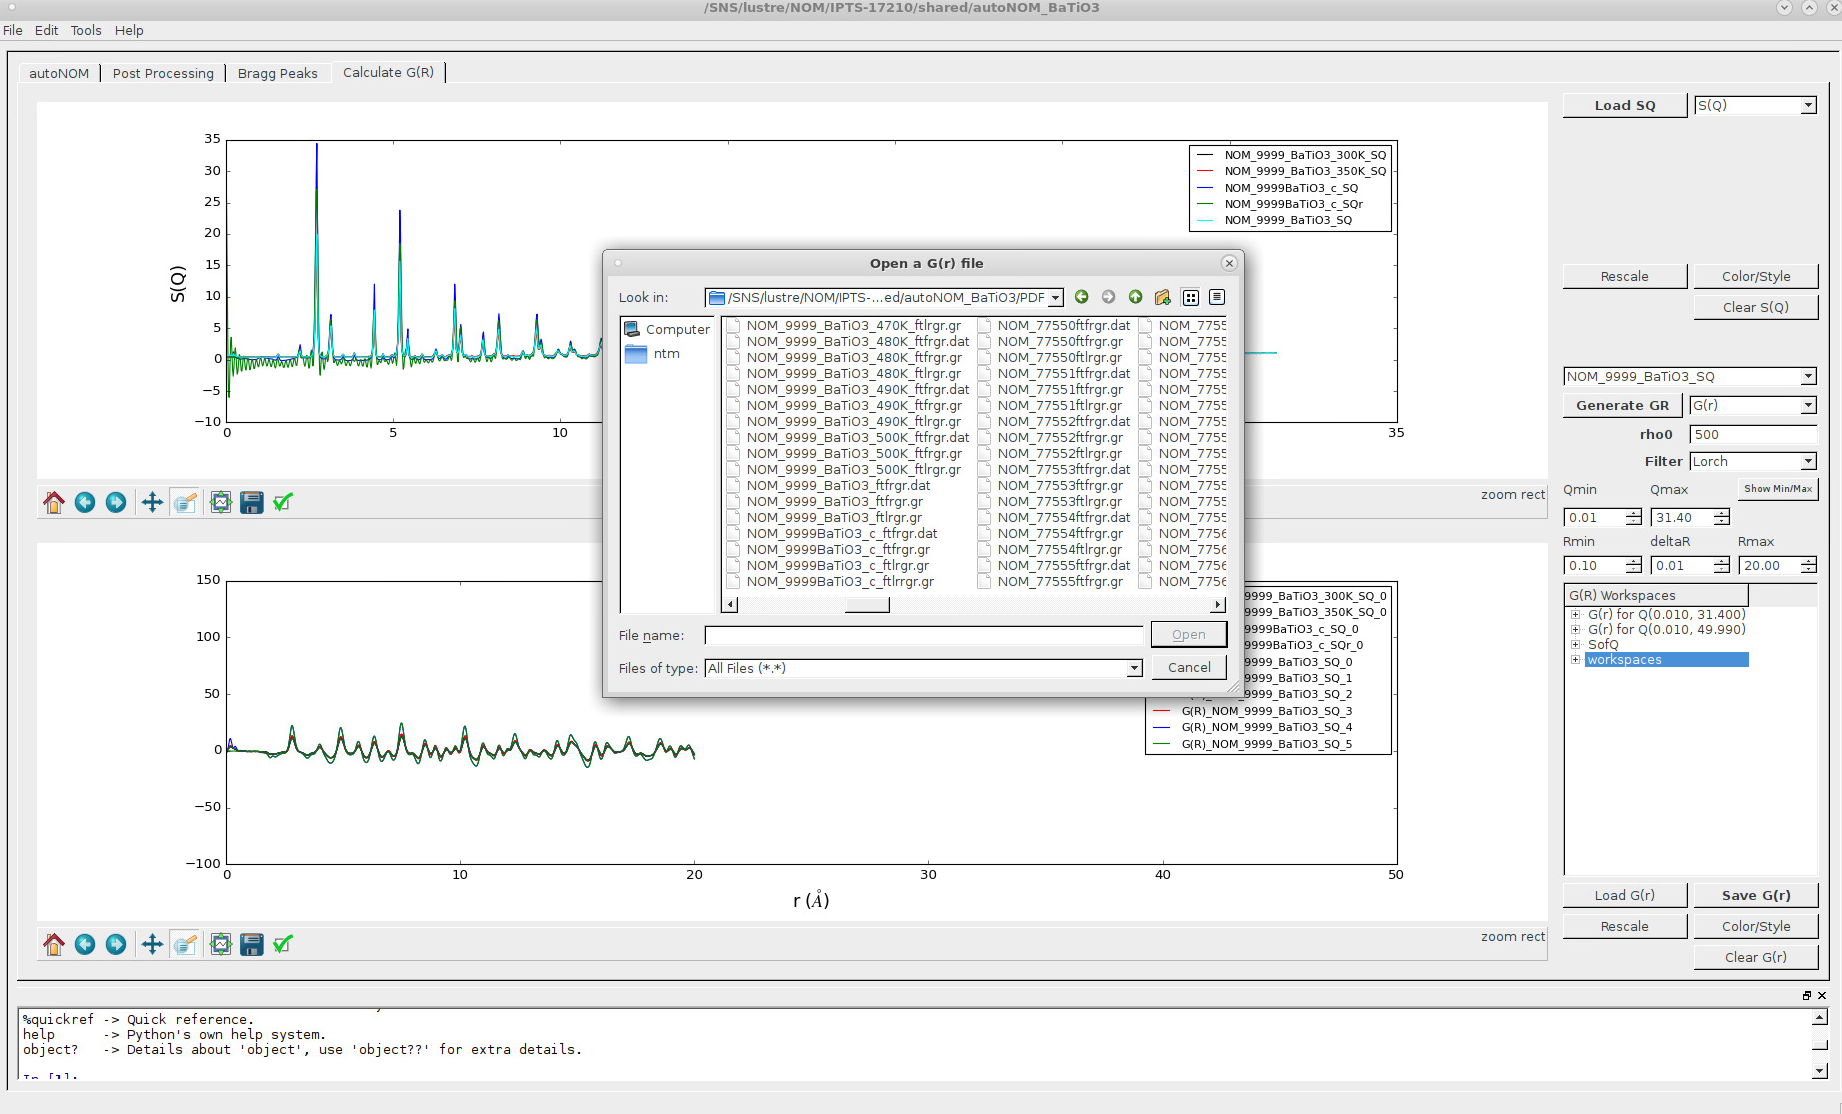
\includegraphics[width=0.9\paperwidth]{graphics/tab4/tab4_populatedGraph_loadGofR.png}}

If you choose the \fileio{gofr}, you should be presented with a file dialog similar to the one below:

\noindent\makebox[\textwidth]{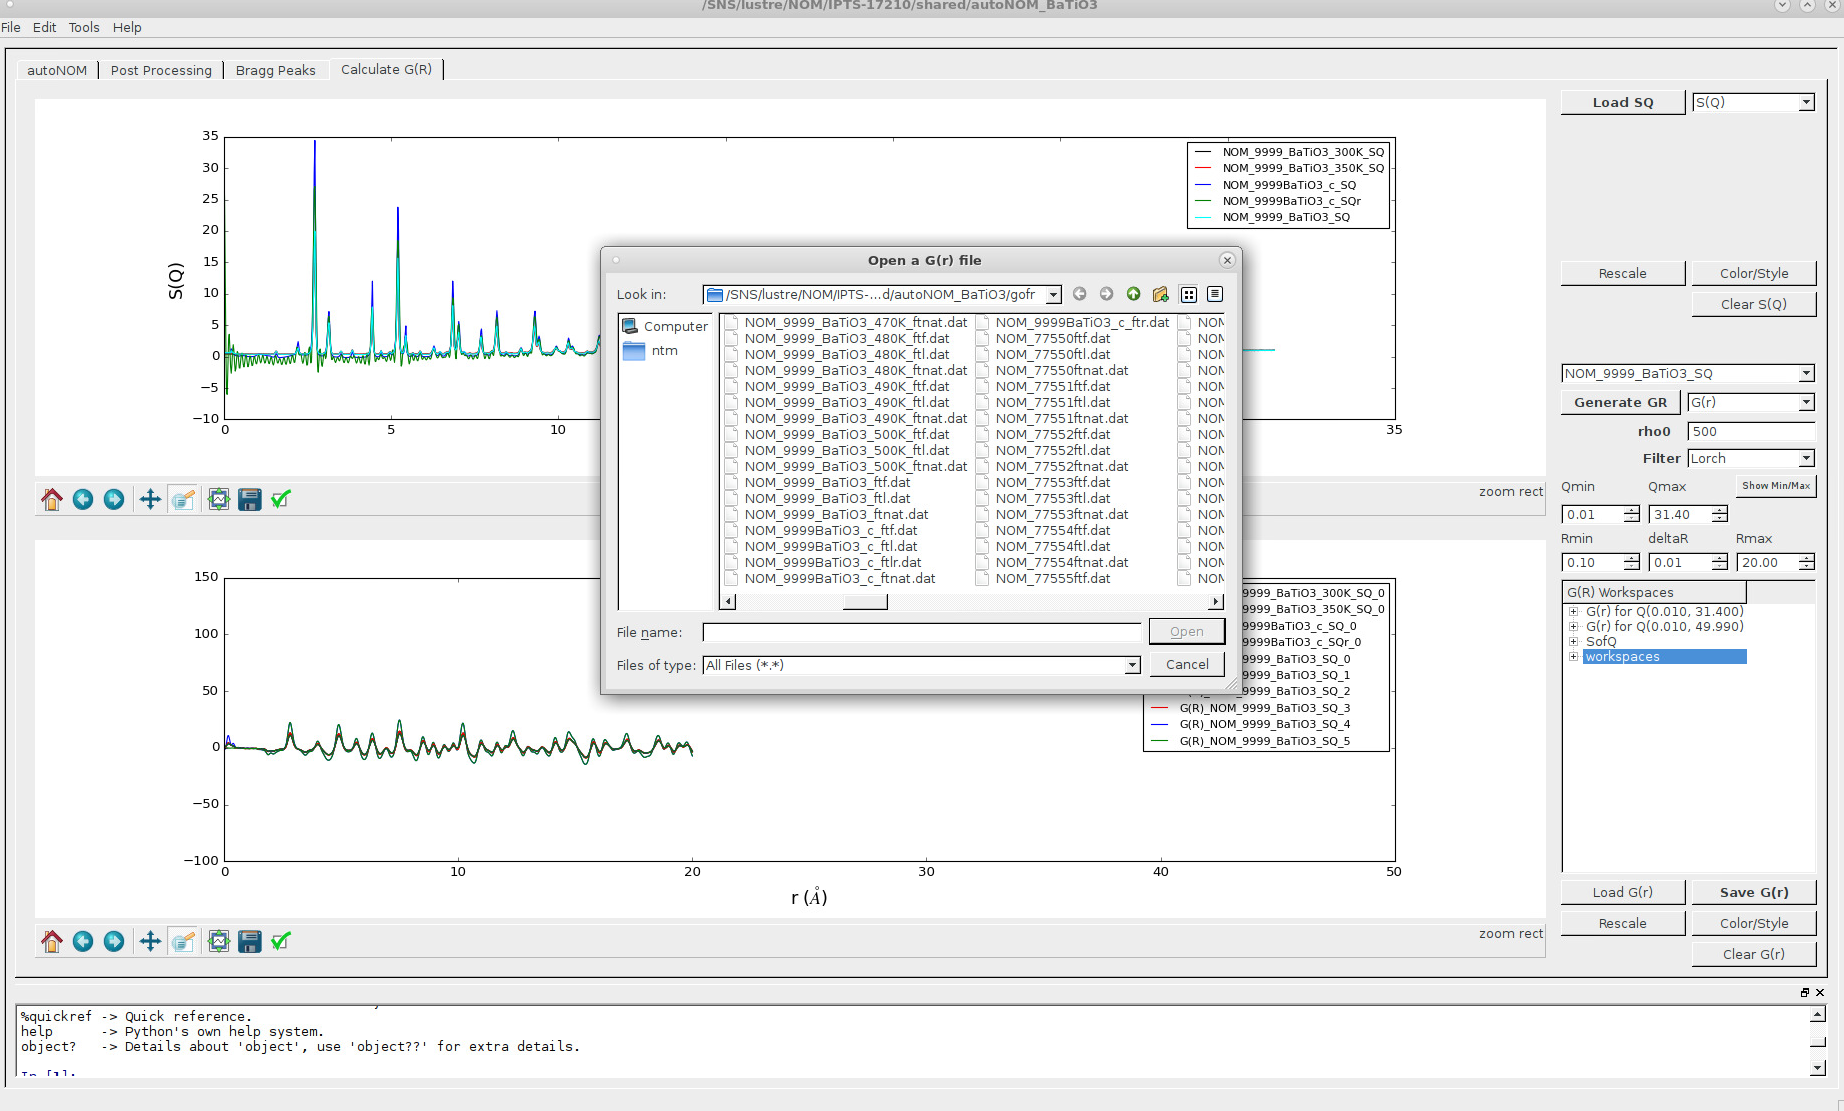
\includegraphics[width=0.9\paperwidth]{graphics/tab4/tab4_populatedGraph_loadGofR_gofr.png}}

For the different file types of both, we have the following:

\begin{itemize}

\item NOMXXXftfrgr.gr – G(r) or PDF of your samples, ready for
analysis for PDFgui software package

\item NOMXXXftlrgr.gr – the same, but convoluted with the
Lorch function 

\item NOMXXXftl.dat, NOMXXXftf.dat – small g(r)

\end{itemize}


\subsection{Output G(r)}
The \guicmd{Save G(r)} button will allow you to output your selected G(r) workspace into a variety for file formats. Currently, you can output it to the following formats:

\noindent\makebox[\textwidth]{\includegraphics[width=0.9\paperwidth]{graphics/tab4/tab4_populatedGraph_saveGofR.png}}


\subsection{Optimize G(r)}

\textbf{Insert the optimization strategies we have discussed for each instrument scientist's method}






\textbf{Add references through manual}

\end{document}
